% !TEX encoding = UTF-8 Unicode
% !BIB TS-program = biber
%
% This file is MIT-Thesis.tex, a LaTeX template for formatting an MIT thesis with the mitthesis class.
%
% Version: 1.20, 2025/05/02
%
% Author: John H. Lienhard, copyright 2025. Reuse under the MIT license: https://ctan.org/license/mit 
%
% Documentation is here: https://ctan.org/pkg/mitthesis


%% Don't modify the \DocumentMetadata command unless you know what it does. 
%% If this command throws an "undefined" error, your latex installation is out of date: try commenting this command out.
\DocumentMetadata 
{
	lang		= en-US,
	pdfversion  = 1.7,
	pdfstandard = a-2b,
%	debug		= {xmp-export}, % if you want to check your metadata (xmpi file).
}

%%%%%%%%%  Documentclass and options  %%%%%%%%%%%%%%%%%%%%%%%%%%%%%%%%%%%%%

\documentclass[twoside]{mitthesis}% fontset=libertinus, fontset=lmodern, fontset=lucida, 
%						fontset=fira-newtxsf, fontset=newtx, fontset=newtx-sans-text,  
%						fontset=heros-stix2,  fontset=stix2, fontset=termes-stix2, fontset=termes
%
% option [twoside]		gives facing-page behavior for printing; omitting twoside will eliminate even-numbered blank pages.
%
% option [lineno]	 	provides line numbers, as for editing
%
% option [fontset=xxx]  is a keyvalue which can be:
%					 	for pdftex or lualatex engine:  defaultfonts, libertinus, lmodern, lucida
%					 	for pdftex only: 				fira-newtxsf, newtx, newtx-sans-text
%						for lualatex only:				heros-stix2, stix2, termes, termes-stix2
%					 	if no key value is given, fonts default to CMR (pdftex) or LMR (unicode), i.e., "the LaTeX font".
%					 	You can edit the fontset files or you can write your own, myfonts.tex, and do [fontset=myfonts].
%						If you are using multiple languages, load the babel package in your fontset file, before the fonts.
%
% option [mydesign] 	loads packages for color, title and list formats, margins, or captions. 
%	or [mydesign=file]	You can edit mydesign.tex to change defaults. Other design files can be loaded as
%						key values, [mydesign=filename], where filename.tex should be in your working directory.
%						Two example files are provided: mydesign_redsans_headings.tex and mydesign_libertinus_headings.
%						See documentation for details and a description of the appropriate fontsets to use with each.						

%%%%%%%%  Packages used in sample chapters (not otherwise required) %%%%%%%

%% Package for code listing in Appendix A.
\usepackage{listings}%   documentation is here https://ctan.org/pkg/listings

%% Set chemical formulas nicely
\usepackage[version=4]{mhchem}%   documentation at https://ctan.org/pkg/mhchem

%% Latin filler used in Chapter 1, with a test for package version date (https://ctan.org/pkg/lipsum)

%%%%%%%%%  Other optional packages used sample chapters  %%%%%%%%%%%%%%%%%%

%% Table related packages  

\usepackage{booktabs}% publication quality tables (https://ctan.org/pkg/booktabs)

\usepackage{array}% Additional options for column formats (https://ctan.org/pkg/array)

\usepackage{dcolumn}% For alignment of numbers on the decimal place (https://ctan.org/pkg/dcolumn) 
  \newcolumntype{d}[1]{D{.}{.}{#1}}% use with dcolumn package. Note: dcolumns are set in math mode.
  % syntax: d{x.y} where x is max number of digits before decimal and y is max number after.

% Package for multipage table in Appendix B.
\usepackage{longtable}% typeset multi-page tables (https://ctan.org/pkg/longtable)

%\usepackage{tabularx}% adjustable-width columns in tabular (https://ctan.org/pkg/tabularx)


%% Package for improved typography
\usepackage{microtype}% typographic fine-tuning (https://ctan.org/pkg/microtype)


%% Load this if using the two-column nomenclature format, \begin{nomenclature*}
\usepackage{multicol}


%%%%%%%%%  Graphics path (to figure files)  %%%%%%%%%%%%%%%%%%%%%%%%%%%%%%%%

%% Can set graphicspath to point to specific directories containing figures (the current directory is searched automatically)
%% For instance, to search a subdirectory of the current directory called "figures" and a parallel directory called "art", set:

\graphicspath{{figures/}} % For details see: https://latexref.xyz/dev/latex2e.html#g_t_005cgraphicspath


%%%%%%%%%  Representative set-up for biblatex  %%%%%%%%%%%%%%%%%%%%%%%%%%%%%

%% biblatex is very powerful, and you can customize most aspects the reference list and citations to suit your needs.
%%   documentation is here: https://ctan.org/pkg/biblatex
%%   cheat sheet is here:   https://tug.ctan.org/info/biblatex-cheatsheet/biblatex-cheatsheet.pdf

%% Numerical citations of references
\usepackage[style=ext-numeric-comp,giveninits=true,maxbibnames=10,sorting=none,language=american]{biblatex}

% and make some changes to that style
	\renewcommand{\multicitedelim}{\addcomma}% removes space between consecutive cites to give [6,7], not [6, 7]
    \AtEveryBibitem{%
      \ifentrytype{article}{%
        \renewbibmacro{in:}{}% Removes "In:" for articles
		\renewcommand*{\jourvoldelim}{\addcomma\space}   % put comma after journal title
		\renewcommand*{\volnumdatedelim}{\addcomma\space}% put comma after volume info
		\renewbibmacro*{issue+date}{% Print date without parentheses around it
		\iffieldundef{issue}%
        	{}%
        	{\printfield{issue}%
         	\setunit*{\addcomma\space}
        	}%
			\printdate
		}
      }{}
    }
	\renewbibmacro*{volume+number+eid}{%
        \printtext[bold]{\printfield{volume}}%    bold volume (issue number) , eid
        \printtext[parens]{\printfield{number}}%  
        \setunit{\bibeidpunct}%
        \printfield{eid}
    }



%% IEEE style citations and references
% \usepackage[style=ieee,maxbibnames=10,sorting=none]{biblatex}% style=ext-numeric-comp,articlein=false,giveninits=true
%	 \DefineBibliographyStrings{english}{url= \textsc{url} ,  }% replaces the IEEE default "[Online]. Available" by "URL"

%% author-year style citations and references 
%% use \parencite, not \cite, when you want "(Author, year)"
%% The sample files are not set up to include parentheses.
% \usepackage[style=authoryear, maxbibnames=10]{biblatex} 


\addbibresource{bibliography.bib}%% <== change to YOUR bib file <= CHANGE


%% to avoid split urls and stretched white space, you can make the bibliography ragged-right by uncommenting this:
%\AddToHook{cmd/bibsetup/after}{\raggedright}

%% To ensure citations are set, run Latex --> biblatex --> Latex again (unless you installation does this automatically)


%%%%%%%%%%  Option for "double spacing" %%%%%%%%%%%%%%%%%%%%%%%%%%%%%%%%%%%%

%% Back in the typewriter era, double spaced lines were convenient for editing with a pencil. 
%% In typography, the separation between lines is called "leading", and it is usually set in 
%% proportion to the font size (i.e., when the font is loaded).  If you really feel the need 
%% to change the line separation, the most attractive results will be obtained by changing the
%% leading in proportion to the the current font size, rather than just doubling the space.

%% The setspace package provides a tool for changing line separation. Use these two commands here:
%
% \usepackage{setspace}%  documentation at https://ctan.org/pkg/setspace
% \setstretch{1.1}% you can choose some other value for the stretch of space between lines
%
%% Use one or more of the these commands *AFTER* the frontmatter
%
% \onehalfspacing
% \doublespacing
% \singlespacing  % will turn these effects off (you can use these anywhere in the document)

%% The best result is usually to stay with the default leading (or to learn about latex font settings).


%%%%%%%%%%%  Metadata  %%%%%%%%%%%%%%%%%%%%%%%%%%%%%%%%%%%%%%%%%%%%%%%%%%%%%%%

% Most of the document metadata is created automatically. 
% The following items should be adjusted to match your work. <================= !!!!!!!!!!

\hypersetup{%
	pdfsubject={Collaboration-Based Learning Environments using Augmented Reality. Thesis document for the title of Doctor of Philosophy in Creative Technologies, Sebastian Gil Parga, 2025.},
	% Change this to briefly state topic of your thesis 
% 
	pdfkeywords={Thesis, AUT, Creative Technologies, Augmented Reality, Learning Environments, Collaborative Learning},
	% Add keywords that will help search engines and libraries to find your work.
	% Includes the name[s] of the author[s] 
	% (If you used \DocumentMetadata at line 14, you can just put "\CopyrightAuthor," for the names.)
%	
	pdfcontactemail={s.gilparga@gmail.com},
	% You can put a [permanent] email address into the metadata, if you like.
	% Otherwise delete this.
%
}

%%%%%%%%%%%%  Math operators %%%%%%%%%%%%%%%%%%%%%%%%%%%%%%%%%%%%%%%%%%%%%%%%%%%%

% These commands declare two math operators, \erf{..} and \erfc{..} using mathtools
% note: * form produces automatic delimiter scaling; optional argument sets size manually, e.g. [\bigg]
% See Table 1.1 in Chapter 1

\DeclareMathOperator{\Erf}{erf}
\DeclareMathOperator{\Erfc}{erfc}
\DeclarePairedDelimiterXPP\erf[1]{\Erf\mkern1mu}(){}{#1}% increase to 2mu with stix2 font
\DeclarePairedDelimiterXPP\erfc[1]{\Erfc\mkern1mu}(){}{#1}


%%%%%%%%%%%%%%  End preamble %%%%%%%%%%%%%%%%%%%%%%%%%%%%%%%%%%%%%%%%%%%%%%%%%%%%%%%%%%%%%%%%%%%%%
%%%%%%%%%%%%%%%%%%%%%%%%%%%%%%%%%%%%%%%%%%%%%%%%%%%%%%%%%%%%%%%%%%%%%%%%%%%%%%%%%%%%%%%%%%%%%%%%%%

\begin{document}
\title{Collaboration-Based Learning Environments using Augmented Reality}

% \Author{Author full name}{Author department}[Author's first PREVIOUS degree][Author's second PREVIOUS degree][...
\Author{Sebastian Gil Parga}{School of Future Environments, Department of Creative Technologies}

\Degree{Doctor of Philosophy in Creative Technologies}{Department of Creative Technologies}

% If there is more than one supervisor, use the \Supervisor command for each.
\Supervisor{Stefan Marks}{Associate Professor}
\Supervisor{Jairo Gutierrez}{Professor}

% Professor who formally accepts theses for your department (e.g., the Graduate Officer, Professor Sméagol,...)
% If more than one department, use more than once
\Acceptor{Tertius Castor}{Professor of Log Dams}{Graduate Officer, Department of Research} % \\ \> Third title}
% \Acceptor{Quarta Castor}{Professor of Lodge Building}{Graduate Officer, Department of Mechanical Engineering}
%%%  If you need to reduce vertical space, put the acceptor title in the second argument and leave the third blank, {}.
% \Acceptor{Primus Castor}{Professor and Undergraduate Officer, Department of Physics}{}

% Usage: \DegreeDate{Month}{year}
% Valid degree months are February, May, June, or September
\DegreeDate{November}{2025}

% Date that final thesis is submitted to department
\ThesisDate{November 30, 2025}


%%%%%%  Choose whether to have a CREATIVE COMMONS License  %%%%%%%%%%%%%%%%%%%%%%%%%%%%%%%%%%%%%%
%
% If you are using a cc license, uncomment the following line and insert details of your cc license here.
%
% \CClicense{CC BY-NC-ND 4.0}{https://creativecommons.org/licenses/by-nc-nd/4.0/}
%

%%%%%%%  Solutions for overflowing titlepage  %%%%%%%%%%%%%%%%%%%%%%%%%%%%%%%%%%%%%%%%%%%%%%%%%%%

% If your title page is overflowing (from too many names, degrees, etc.):
%
% (a) you can reduce the 12pt and 18pt skips between various blocks to 6pt with this command:
%
% \Tighten
%
% (b)  you can scale down the Signature block at the bottom with this command:
%
% \SignatureBlockSize{\small}  %or this one \SignatureBlockSize{\footnotesize}
%
% (c) you can put the acceptor name and title onto two lines, rather than three like this:
%
% \Acceptor{Tertius Castor}{Professor and Graduate Officer, Department of Research}{}
%
% (d) you can change the font size of the author name[s] with
%
%	\AuthorNameSize{\normalsize}
%
% (e) and you can omit any previous degrees from the title page, instead mentioning them in the biographical sketch

% Also, if you prefer to keep the text toward the top of the page with most white space at the bottom, you
% can use this command to squash all of the vertical glue (stretchy space) with this command:
%
% \Squash 
%
% This command is useful when the text has not already reach the bottom of the page, since the glue gets squashed automatically
% when the page is too full.

%%%%%%%%%%%%%%%%%%%%%%%%%%%%%%%%%%%%%%%%%%%%%%%%%%%%%%%%%%%%%%%%%%%%%%%%%%%%%%%%%%%%%%%%%%%%%%%%%


%%% Make titlepage
\maketitle


%%%%%%%%% Content that you need to write follows! %%%%%%%%%%%%%%%%%%%%%%%%%%%%%%%%%%%%%%%%%%%%%%

% \includeonly{acknowledgments,biography,chapter1,chapter2,...,appendixa,...} 
%   for usage of includeonly, see https://latexref.xyz/_005cinclude-_0026-_005cincludeonly.html


%%% Frontmatter (write this material in the mentioned files)  %%%%%%%%%%%%%%%%%%%%%%%%%%%%%%%%%%%

% Sample thesis committee page for mitthesis.cls
% Version 1.03, 2025/05/01
%
% This page is not required by the MIT Libraries, but some departments require it.
%
% Insert between title page and abstract page.
% Format this page in any way that you like (no specific requirements exist)
% 
% Add supervisor titles, degrees, and departments as appropriate, starting at line 32.


%%%%%  Formatting commands (you can ignore these)  %%%%%%%%%%%%%%%%%%

%% format this chapter title
\newcommand\CMstyle[1]{\pdfbookmark[0]{#1}{thesiscommittee}\bfseries\Large\lsstyle \MakeUppercase{#1}}

\newcommand\CMsubstyle[1]{\pdfbookmark[1]{#1}{#1}\flushright\normalfont\scshape\large\lsstyle #1}

%   \lsstyle produces additional letter separation (appropriate for capitalized display text),
% 	when \usepackage{microtype} has been given in the preamble. 
% 	If microtype has not been loaded, mitthesis.cls will ignore this command.
% 	The extra space added between letters is 100/1000 em (adjustable, see microtype documentation).


%%%%%%%%%%  EDIT THE NAMES AND TITLES IN THIS PART  %%%%%%%%%%%%%%%%%%%%%%%%%%%%%%%%%%%

\chapter*{\CMstyle{Thesis Committee}}

\section*{\CMsubstyle{Thesis Supervisor}}
\begin{flushright}

 \textbf{Marcus Gavius Apicius} \\ %% <======= edit these lines! 
 {\itshape
  Professor of Cooking Arts \\
  Department of Food Science \\
 }

\end{flushright}


\section*{\CMsubstyle{Thesis Readers}}
\begin{flushright}

 \textbf{Marie-Antoine Carême} \\ %% <======= edit these lines! 
 {\itshape
   Professor of Haute Cuisine \\
   Department of Food Science \\[18pt]
 }

 \textbf{Julia Child} \\ %% <======= edit these lines! 
 {\itshape
   Professor of French Cuisine \\
   Department of Food Science \\[18pt]
 }

 \textbf{Miles Gloriosus} \\ %% <======= edit these lines! 
 {\itshape
   Professor of Personal Pronouns \\
   Department of Rhetoric \\
 }

\end{flushright}
% This page is optional. Edit the file committee_members.tex 

% The abstract environment creates all the required headings and footers. 
% You only need to the text of the abstract in the file abstract.tex
\begin{abstract}
	% From mitthesis package
% Version: 1.01, 2023/06/19
% Documentation: https://ctan.org/pkg/mitthesis
%
% The abstract environment creates all the required headers and footnote. 
% You only need to add the text of the abstract itself.
%
% Approximately 500 words or less; try not to use formulas or special characters
% If you don't want an initial indentation, do \noindent at the start of the abstract

The developments of the ``kinetic theory'' of gases made within the last ten years have enabled it to account satisfactorily for many of the laws of gases. The mathematical deductions of Clausius, Maxwell and others, based upon the hypothesis of a gas composed of molecules acting upon each other at impact like perfectly elastic spheres, have furnished expressions for the laws of its elasticity, viscosity, conductivity for heat, diffusive power and other properties. For some of these laws we have experimental data of value in testing the validity of these deductions and assumptions. Next to the elasticity, perhaps the phenomena of the viscosity of gases are best adapted to investigation.\footnote{Text from Holman (1876): \doi{10.2307/25138434}.}  
% use \input rather than \include because we're inside an environment
\end{abstract}

%% acknowledgments.tex

% From mitthesis package
% Version: 1.02, 2024/06/19
% Documentation: https://ctan.org/pkg/mitthesis

\chapter*{Acknowledgments}
\pdfbookmark[0]{Acknowledgments}{acknowledgments}


Write your acknowledgments here.
% acknowledgments.tex (.tex extension is presumed by \include) 

%% biography.tex
%% This section is optional

% From mitthesis package
% Version: 1.02, 2024/06/19
% Documentation: https://ctan.org/pkg/mitthesis

\chapter*{Biographical Sketch}
\pdfbookmark[0]{Biographical Sketch}{biosketch}


Silas Whitcomb Holman was born in Harvard, Massachusetts on January 20, 1856. He received his S.B. degree in Physics from MIT in 1876, and then joined the MIT Department of Physics as an Assistant. He became Instructor in Physics in 1880, Assistant Professor in 1882, Associate Professor in 1885, and Full Professor in 1893. Throughout this period, he struggled with increasingly severe rheumatoid arthritis. At length, he was defeated, becoming Professor Emeritus in 1897 and dying on April 1, 1900.

Holman's light burned brilliantly before his tragic and untimely death. He published extensively in thermal physics, and authored textbooks on precision measurement, fundamental mechanics, and other subjects. He established the original Heat Measurements Laboratory. Holman was a much admired teacher among both his students and his colleagues. The reports of his department and of the Institute itself refer to him frequently in the 1880's and 1890's, in tones that gradually shift from the greatest respect to the deepest sympathy.

Holman was a student of Professor Edward C. Pickering, then head of the Physics department. Holman himself became second in command of Physics, under Professor Charles R. Cross, some years later. Among Holman's students, several went on to distinguish themselves, including: the astronomer George E. Hale ('90) who organized the Yerkes and Mt. Wilson observatories and who designed the 200 inch telescope on Mt. Palomar; Charles G. Abbot ('94), also an astrophysicist and later Secretary of the Smithsonian Institution; and George K. Burgess ('96), later Director of the Bureau of Standards. % biography.tex (optional, see https://libraries.mit.edu/distinctive-collections/thesis-specs/#format)

%%% Table of contents and lists of stuff (delete unused lists, i.e., if no tables or figures) %%%%%

\tableofcontents
\listoffigures
\listoftables

%%% Chapters of thesis  %%%%%%%%%%%%%%%%%%%%%%%%%%%%%%%%%%%%%%%%%%%%%%%%%%%%%%%%%%%%%%%%%%%%%%%%%%%

%% If you want to use "double spacing", you should start here...

 \chapter{Introduction}

In the Netflix animated series Cyberpunk: Edgerunners \parencite{cyberpunk_2022}, the main character attends courses at a 
prestigious academy that uses advanced technology to boost education and performance. The students gather in a room with
Virtual Reality \ac{VR} headsets and connect to the lesson, which is taught by a holographic (and probably powered by artificial
intelligence) tutor. The episode does not show the lesson itself (the entire system fails catastrophically when attacked by
malware), but the brief scene highlights the vision many people have of a futuristic classroom, one guided by advanced technology
and automatization.

\begin{figure}[t]
    \centering{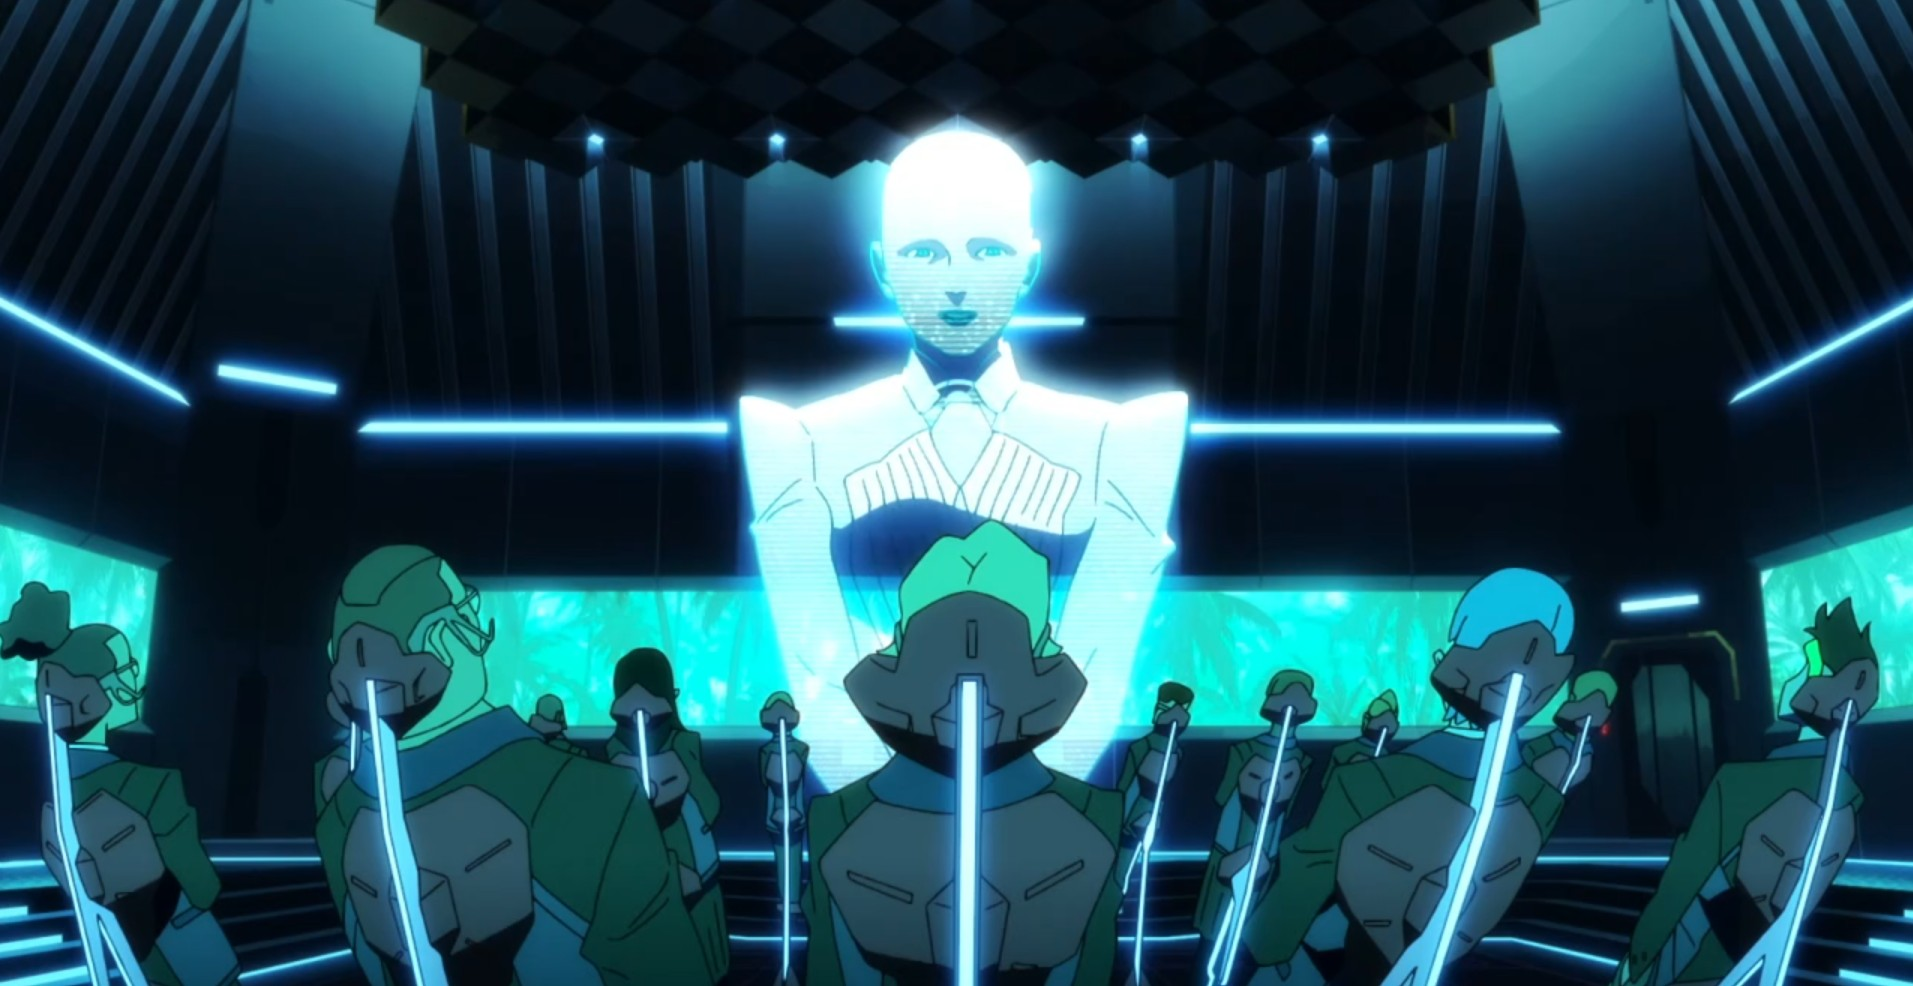
\includegraphics[alt={Figure 1.1},width=0.99\textwidth]{figures/F1-1.jpg}}
    \caption{Virtual Classroom in Cyberpunk: Edgerunners\label{fig:1-1}}
\end{figure}

\textcite{forsler_2024} propose the term “post-digital classroom” to identify the characteristics and trends in education
present in a world beyond the adoption of digital technologies. The purpose of this classroom is not anymore to
introduce new technologies to students, but to implement them as an essential factor of the learning process. The
post-digital classroom is interconnected, social and global. In this scenario, learning goes beyond the physical
classroom because it is based on creating relationships between concepts and developing valuable skills rather than
acquiring knowledge. It is also a classroom where information is detached from the physical learning institute, and
access to facts and sources is, ideally, immediate, ubiquitous and democratic.

The classroom has also become hybrid. There is little distinction between network-based lessons and the face-to-face spaces
associated with schools and universities \parencite{goodyear_2004}. Hybrid and blended approaches blur the distinctions
between learning in an online setting and learning in a classroom. In both instances, information is at hand in the network,
students can easily connect to peers and mentors, distance and time constrains are less meaningful and knowledge is presented
in a multimedia format that needs a technological backbone to be created and shared \parencite{rivoltella_2008,shank_2005}.

This thesis explores the use of technology in such post-digital classrooms, specifically, Augmented Reality \ac{AR} within the
context of mobile computing. Moreover, this research will analyse the creation of effective learning spaces, those places where
students can build, personalise and control all the activities they engage with \parencite{gourlay_2016}. Learning spaces are
interesting tools at the disposal of students because these are spaces that can exist outside the norm of a typical classroom,
they are more fluid, less structured and can easily connect to other similar spaces \parencite{norgard_2022}. The proposal of
this research is that \ac{AR} can be used to boost the way students build and interact with their own learning spaces and can also
offer educators another option to be integrated in the construction of a lesson that capitalises the characteristics of the
aforementioned post-digital classrooms.

Within the field of Technology Enhanced Learning \ac{TEL}, \ac{AR} and related technologies were chosen as a focus of interest
because of their intrinsic relationship with space. The initial example scene of Cyberpunk: Edgerunners serves to illustrate the
collective idea of what could be achieved in the future with technologies like \ac{VR} and \ac{AR}: the possibility of creating an
entire new space, suited for the needs of the classroom or the students. It is a space that is shared, in which information and
interactions flow between users and that can be controlled at will by students and teachers. In reality, the technology is not quite
there yet, especially in terms of fidelity and immersion \parencite{hamad_2022,checa_2020}. What can be explored right now is the
creation of interesting synthetic environments that facilitate or allow experiences that are not possible in the common classroom.
This process is limited more by the creativity and expertise of the developer rather than by the technology, and therefore can be
explored easier and in more detail.

\ac{AR}, compared to \ac{VR}, has a more direct relationship with the \emph{real}, physical space and with the context of the user.
Instead of an isolated immersion, \ac{AR} creates a connection with the environment based on image detection, data and visualizations.
This natural expression of the technology is where the value of \ac{AR} can be explored in relation to the creation of innovative
learning spaces. The technology not only has interesting capabilities for visualization and interaction, it also allows an easier
implementation of shared, social components that can be used to build activities based on cooperative simulations, sharing knowledge and
the creation of communities, all crucial elements for the construction of effective learning spaces \parencite{bligh_2017}.

The research is positioned then in the conjunction of these three fields: Learning spaces, \ac{TEL} and \ac{AR}. The guiding goal is to
understand how students are using technology to learn, and how \ac{AR} can be used to boost that process. \ac{AR} shines at creating
immersive experiences that can be shared with others and that consider the physical context of the user. I want to use this collaborative
space as an educational tool that takes advantage of the inherent social aspects of learning, building and sharing knowledge.

\section[Context]{Context}

\section[Research Structure]{Research Structure}
\subsection[Research Questions]{Research Questions}
\subsection[Scope and Limitations]{Scope and Limitations}
\section[Significance and Contributions]{Significance and Contributions}
\section[Document Structure]{Document Structure}% .tex extension is presumed
% \include{chapter2}
% \include{chapter3}
% \include{chapter4}


%%% Appendicies of thesis  %%%%%%%%%%%%%%%%%%%%%%%%%%%%%%%%%%%%%%%%%%%%%%%%%%%%%%%%%%%%%%%%%%%%%%%%

\appendix
% From mitthesis package
% Version: 1.01, 2023/07/04
% Documentation: https://ctan.org/pkg/mitthesis


\chapter{Code listing}

This example uses the \texttt{listings} package.

\bigskip

\lstdefinestyle{mystyle}{
    backgroundcolor=\color{CadetBlue!15!white},   
    commentstyle=\color{Red3},
    numberstyle=\tiny\color{gray},
    stringstyle=\color{Blue3},
    basicstyle=\small\ttfamily,
    breakatwhitespace=false,         
    breaklines=true,                 
    numbers=left,                    
    numbersep=5pt,                  
    showspaces=false,                
    showstringspaces=false,
    showtabs=false,                  
    tabsize=2
}%
\lstset{language=[5.3]Lua,style={mystyle}}%

\begin{lstlisting}
function print_rate(kappa,xMin,xMax,npoints,option)
     local c = 1-kappa*kappa
     local croot = (1-kappa*kappa)^(1/2)
     local logx = math.log(xMin)
     local psi = 0
     
     local xstep = (math.log(xMax)-math.log(xMin))/(npoints-1)
     
     arg0 = math.sqrt(xMin/c)
     psi0 = (1/c)*math.exp((kappa*arg0)^2)*(erfc(kappa*arg0)-erfc(arg0))
     
     if option~=[[]] then
  		 tex.sprint("\\addplot+["..option.."] coordinates{") 
  		 -- addplot+ for color cycle to work
     else
  		 tex.sprint("\\addplot+ coordinates{")
     end
     tex.sprint("("..xMin..","..psi0..")")
     
     for i=1, (npoints-1) do
  		 x = math.exp(logx + xstep)
  		 arg = math.sqrt(x/c)
  		 karg = kappa*arg
  		 if karg<5 then 
		 -- this break compensates for exp(karg^2), which multiplies the error in the erf approximation...
  		    logpsi = -math.log(croot) + karg^2 + math.log(erfc(karg)-erfc(arg))
  		    psi = math.exp(logpsi)
  		 else
  		    psi = (1/(karg) - 1/(2*(karg^3)) + 3/(4*(arg^5)) )/(1.77245385*croot)
  		    -- this is the large x asymptote of the reaction rate
  		 end
  		 logx = math.log(x)
  		 tex.sprint("("..x..","..psi..")")
     end
     tex.sprint("}")
end
\end{luacode*}
\end{lstlisting}
% listings example
%% MIT Thesis class sample appendix with a long table
%% version 1.02, 2024/09/07

\chapter{One-term coefficients for heat conduction}

\section{A multipage table of numbers}
This example uses the \texttt{longtable} package: $\theta = A_1 f_1 \exp(-\lambda_1^2\mkern2mu\mathrm{Fo})$, $\overline{\theta} = D_1 \exp(-\lambda_1^2\mkern2mu\mathrm{Fo})$.


%% These four lines change the dcolumn to use text figures, instead of math figures.
%% The reason is that some mitthesis font sets use different typefaces for text and math
%% See: https://tex.stackexchange.com/a/376127/119566
\makeatletter
	\newcolumntype{T}[3]{>{\textfont0 =\the\font\DC@{#1}{#2}{#3}}c<{\DC@end}}
	\newcolumntype{d}[1]{T{.}{.}{#1}}% overwrites definition in root .tex file + gives warning message
\makeatother

{\footnotesize
% read documentation of longtable package for info on setting up a long table
% read documentation of array package and dcolumn package for info on column format specifiers
\renewcommand{\doublerulesep}{0pt}%
\newcolumntype{X}{>{\hspace{1ex}}c@{\hspace{2ex}}c@{\hspace{2ex}}c<{\hspace{1ex}}}%

\begin{longtable}{|||d{3.2}|X|X|X|||}

\caption{One-term coefficients for one-dimensional heat conduction with a convective boundary condition. Data follow H. D. Baehr and K. Stephan~\cite{baehr1998}.}%

\\
\hline\hline\hline
&&&&&&&&&\\[-7pt]
& \multicolumn{3}{c|}{\textsf{\textit{Plate}}} & \multicolumn{3}{c|}{\textsf{\textit{Cylinder}}} & \multicolumn{3}{c|||}{\textsf{\textit{Sphere}}}
\\ 
\cline{2-10} 
\multicolumn{1}{|||c|}{\raisebox{1.5ex}[0cm][0cm]{Bi}} 
       & $\lambda_1$\rule[0pt]{0pt}{11pt} & $A_1$ & $D_1$ & $\lambda_1$ & $A_1$ & $D_1$ & $\lambda_1$ & $A_1$ & $D_1$ 
\\  
\hline  
\endfirsthead
\caption[]{(continued)} \\
\hline\hline\hline
&&&&&&&&&\\[-7pt]
& \multicolumn{3}{c|}{\textsf{\textit{Plate}}} & \multicolumn{3}{c|}{\textsf{\textit{Cylinder}}} & \multicolumn{3}{c|||}{\textsf{\textit{Sphere}}}
\\ 
\cline{2-10}
\multicolumn{1}{|||c|}{\raisebox{1.5ex}[0cm][0cm]{Bi}} 
       & $\lambda_1$\rule[0pt]{0pt}{11pt} & $A_1$ & $D_1$ & $\lambda_1$ & $A_1$ & $D_1$ & $\lambda_1$ & $A_1$ & $D_1$ 
\\ \hline
&&&&&&&&&\\[-1ex]
\endhead
\hline\hline\hline
\endfoot
\hline\hline\hline
\endlastfoot 
0.01   & 0.09983  & 1.0017  & 1.0000  & 0.14124   & 1.0025  & 1.0000  & 0.17303  & 1.0030  & 1.0000\rule[0pt]{0pt}{15pt} \\ 
0.02   & 0.14095  & 1.0033  & 1.0000  & 0.19950   & 1.0050  & 1.0000  & 0.24446  & 1.0060  & 1.0000 \\ 
0.03   & 0.17234  & 1.0049  & 1.0000  & 0.24403   & 1.0075  & 1.0000  & 0.29910  & 1.0090  & 1.0000 \\ 
0.04   & 0.19868  & 1.0066  & 1.0000  & 0.28143   & 1.0099  & 1.0000  & 0.34503  & 1.0120  & 1.0000 \\  
0.05   & 0.22176  & 1.0082  & 0.9999  & 0.31426   & 1.0124  & 0.9999  & 0.38537  & 1.0150  & 1.0000 \\  
0.06   & 0.24253  & 1.0098  & 0.9999  & 0.34383   & 1.0148  & 0.9999  & 0.42173  & 1.0179  & 0.9999 \\   
0.07   & 0.26153  & 1.0114  & 0.9999  & 0.37092   & 1.0173  & 0.9999  & 0.45506  & 1.0209  & 0.9999 \\  
0.08   & 0.27913  & 1.0130  & 0.9999  & 0.39603   & 1.0197  & 0.9999  & 0.48600  & 1.0239  & 0.9999 \\  
0.09   & 0.29557  & 1.0145  & 0.9998  & 0.41954   & 1.0222  & 0.9998  & 0.51497  & 1.0268  & 0.9999 \\  
0.10   & 0.31105  & 1.0161  & 0.9998  & 0.44168   & 1.0246  & 0.9998  & 0.54228  & 1.0298  & 0.9998 \\[6pt]   
%
0.15   & 0.37788  & 1.0237  & 0.9995  & 0.53761   & 1.0365  & 0.9995  & 0.66086  & 1.0445  & 0.9996 \\*  
0.20   & 0.43284  & 1.0311  & 0.9992  & 0.61697   & 1.0483  & 0.9992  & 0.75931  & 1.0592  & 0.9993 \\  
0.25   & 0.48009  & 1.0382  & 0.9988  & 0.68559   & 1.0598  & 0.9988  & 0.84473  & 1.0737  & 0.9990 \\  
0.30   & 0.52179  & 1.0450  & 0.9983  & 0.74646   & 1.0712  & 0.9983  & 0.92079  & 1.0880  & 0.9985 \\  
0.40   & 0.59324  & 1.0580  & 0.9971  & 0.85158   & 1.0931  & 0.9970  & 1.05279  & 1.1164  & 0.9974 \\  
0.50   & 0.65327  & 1.0701  & 0.9956  & 0.94077   & 1.1143  & 0.9954  & 1.16556  & 1.1441  & 0.9960 \\ 
0.60   & 0.70507  & 1.0814  & 0.9940  & 1.01844   & 1.1345  & 0.9936  & 1.26440  & 1.1713  & 0.9944 \\  
0.70   & 0.75056  & 1.0918  & 0.9922  & 1.08725   & 1.1539  & 0.9916  & 1.35252  & 1.1978  & 0.9925 \\  
0.80   & 0.79103  & 1.1016  & 0.9903  & 1.14897   & 1.1724  & 0.9893  & 1.43203  & 1.2236  & 0.9904 \\  
0.90   & 0.82740  & 1.1107  & 0.9882  & 1.20484   & 1.1902  & 0.9869  & 1.50442  & 1.2488  & 0.9880 \\[6pt]  
%
1.00   & 0.86033  & 1.1191  & 0.9861  & 1.25578   & 1.2071  & 0.9843  & 1.57080  & 1.2732  & 0.9855 \\* 
1.10   & 0.89035  & 1.1270  & 0.9839  & 1.30251   & 1.2232  & 0.9815  & 1.63199  & 1.2970  & 0.9828 \\  
1.20   & 0.91785  & 1.1344  & 0.9817  & 1.34558   & 1.2387  & 0.9787  & 1.68868  & 1.3201  & 0.9800 \\ 
1.30   & 0.94316  & 1.1412  & 0.9794  & 1.38543   & 1.2533  & 0.9757  & 1.74140  & 1.3424  & 0.9770 \\  
1.40   & 0.96655  & 1.1477  & 0.9771  & 1.42246   & 1.2673  & 0.9727  & 1.79058  & 1.3640  & 0.9739 \\  
1.50   & 0.98824  & 1.1537  & 0.9748  & 1.45695   & 1.2807  & 0.9696  & 1.83660  & 1.3850  & 0.9707 \\ 
1.60   & 1.00842  & 1.1593  & 0.9726  & 1.48917   & 1.2934  & 0.9665  & 1.87976  & 1.4052  & 0.9674 \\  
1.70   & 1.02725  & 1.1645  & 0.9703  & 1.51936   & 1.3055  & 0.9633  & 1.92035  & 1.4247  & 0.9640 \\* 
1.80   & 1.04486  & 1.1695  & 0.9680  & 1.54769   & 1.3170  & 0.9601  & 1.95857  & 1.4436  & 0.9605 \\*  
1.90   & 1.06136  & 1.1741  & 0.9658  & 1.57434   & 1.3279  & 0.9569  & 1.99465  & 1.4618  & 0.9570 \\[6pt]  
%
2.00   & 1.07687  & 1.1785  & 0.9635  & 1.59945   & 1.3384  & 0.9537  & 2.02876  & 1.4793  & 0.9534 \\*  
2.20   & 1.10524  & 1.1864  & 0.9592  & 1.64557   & 1.3578  & 0.9472  & 2.09166  & 1.5125  & 0.9462 \\  
2.40   & 1.13056  & 1.1934  & 0.9549  & 1.68691   & 1.3754  & 0.9408  & 2.14834  & 1.5433  & 0.9389 \\  
2.60   & 1.15330  & 1.1997  & 0.9509  & 1.72418   & 1.3914  & 0.9345  & 2.19967  & 1.5718  & 0.9316 \\  
2.80   & 1.17383  & 1.2052  & 0.9469  & 1.75794   & 1.4059  & 0.9284  & 2.24633  & 1.5982  & 0.9243 \\ 
3.00   & 1.19246  & 1.2102  & 0.9431  & 1.78866   & 1.4191  & 0.9224  & 2.28893  & 1.6227  & 0.9171 \\     
3.50   & 1.23227  & 1.2206  & 0.9343  & 1.85449   & 1.4473  & 0.9081  & 2.38064  & 1.6761  & 0.8995 \\     
4.00   & 1.26459  & 1.2287  & 0.9264  & 1.90808   & 1.4698  & 0.8950  & 2.45564  & 1.7202  & 0.8830 \\*   
4.50   & 1.29134  & 1.2351  & 0.9193  & 1.95248   & 1.4880  & 0.8830  & 2.51795  & 1.7567  & 0.8675 \\*    
5.00   & 1.31384  & 1.2402  & 0.9130  & 1.98981   & 1.5029  & 0.8721  & 2.57043  & 1.7870  & 0.8533 \\[6pt]    
%
6.00   & 1.34955  & 1.2479  & 0.9021  & 2.04901   & 1.5253  & 0.8532  & 2.65366  & 1.8338  & 0.8281 \\*     
7.00   & 1.37662  & 1.2532  & 0.8932  & 2.09373   & 1.5411  & 0.8375  & 2.71646  & 1.8673  & 0.8069 \\    
8.00   & 1.39782  & 1.2570  & 0.8858  & 2.12864   & 1.5526  & 0.8244  & 2.76536  & 1.8920  & 0.7889 \\     
9.00   & 1.41487  & 1.2598  & 0.8796  & 2.15661   & 1.5611  & 0.8133  & 2.80443  & 1.9106  & 0.7737 \\     
10.00  & 1.42887  & 1.2620  & 0.8743  & 2.17950   & 1.5677  & 0.8039  & 2.83630  & 1.9249  & 0.7607 \\     
12.00  & 1.45050  & 1.2650  & 0.8658  & 2.21468   & 1.5769  & 0.7887  & 2.88509  & 1.9450  & 0.7397 \\     
14.00  & 1.46643  & 1.2669  & 0.8592  & 2.24044   & 1.5828  & 0.7770  & 2.92060  & 1.9581  & 0.7236 \\     
16.00  & 1.47864  & 1.2683  & 0.8541  & 2.26008   & 1.5869  & 0.7678  & 2.94756  & 1.9670  & 0.7109 \\*     
18.00  & 1.48830  & 1.2692  & 0.8499  & 2.27556   & 1.5898  & 0.7603  & 2.96871  & 1.9734  & 0.7007 \\*     
20.00  & 1.49613  & 1.2699  & 0.8464  & 2.28805   & 1.5919  & 0.7542  & 2.98572  & 1.9781  & 0.6922 \\[6pt]     
%
25.00  & 1.51045  & 1.2710  & 0.8400  & 2.31080   & 1.5954  & 0.7427  & 3.01656  & 1.9856  & 0.6766 \\*     
30.00  & 1.52017  & 1.2717  & 0.8355  & 2.32614   & 1.5973  & 0.7348  & 3.03724  & 1.9898  & 0.6658 \\     
35.00  & 1.52719  & 1.2721  & 0.8322  & 2.33719   & 1.5985  & 0.7290  & 3.05207  & 1.9924  & 0.6579 \\     
40.00  & 1.53250  & 1.2723  & 0.8296  & 2.34552   & 1.5993  & 0.7246  & 3.06321  & 1.9942  & 0.6519 \\    
50.00  & 1.54001  & 1.2727  & 0.8260  & 2.35724   & 1.6002  & 0.7183  & 3.07884  & 1.9962  & 0.6434 \\     
60.00  & 1.54505  & 1.2728  & 0.8235  & 2.36510   & 1.6007  & 0.7140  & 3.08928  & 1.9974  & 0.6376 \\     
80.00  & 1.55141  & 1.2730  & 0.8204  & 2.37496   & 1.6013  & 0.7085  & 3.10234  & 1.9985  & 0.6303 \\    
100.00 & 1.55525  & 1.2731  & 0.8185  & 2.38090   & 1.6015  & 0.7052  & 3.11019  & 1.9990  & 0.6259 \\*    
200.00 & 1.56298  & 1.2732  & 0.8146  & 2.39283   & 1.6019  & 0.6985  & 3.12589  & 1.9998  & 0.6170 \\*    
\infty & 1.57080  & 1.2732  & 0.8106  & 2.40483   & 1.6020  & 0.6917  & 3.14159  & 2.0000  & 0.6079 \\[3pt] 
\end{longtable}
}
% longtable example


%%% Bibliography (biblatex)  %%%%%%%%%%%%%%%%%%%%%%%%%%%%%%%%%%%%%%%%%%%%%%%%%%%%%%%%%%%%%%%%%%%%%%

\defbibheading{bibintoc}{\chapter*{#1}\addcontentsline{toc}{backmatter}{\refname}} 
% this sets the title of contents name for bibliography to \refname (= References)
% change "backmatter" to "chapter" if you prefer a bold face entry in the table of contents

\printbibliography[title={\refname},heading=bibintoc]

% biblatex also supports chapter-by-chapter bibliography, https://tex.stackexchange.com/a/296502/119566
% see the biblatex manual, section 3.14.3


\end{document} 
 